\chapter{スカラー場の転がりによるインフレーション}

\lectureoverview{前回の講義から残された問いが、組織化の方程式
\(\ddot\phi+3H\dot\phi=-V'(\phi)\)を与える。何が動くのか、何が力を及ぼすのか、なぜ膨張が摩擦のように見えるのか。まず固定された箱の中で方程式を導き、次に膨張する箱の中で導く。これをフリードマン方程式と結合するとスローロール機構が得られ、そこでは高くて浅いスカラーポテンシャルがほぼ指数関数的な膨張を駆動する。インフレーションはモノポールを希釈し、幾何を滑らかにする。その終わりには宇宙が再加熱され、従来の熱いビッグバンが始まる。すると最後の問題は避けられない。インフレーションがこれほど効率的に滑らかにするなら、構造はどこから来たのか。一次元のコースティック計算は、微小な速度変動がどのようにシート、フィラメント、結び目を作るかを示す。ただしそれらの変動の量子的起源については次回の講義に先送りする。}

\section{何が何に作用しているのか}

冒頭の問いは方程式
\begin{equation}
\ddot\phi+3H\dot\phi
=F(\phi)
=-\frac{dV}{d\phi}
\label{eq:c09-opening}
\end{equation}
を思い起こさせ、どのような種類の力\(F\)が場に作用しうるのかを問う。この問いは周辺的なものではない。これに答えるには場の力学を再構成しなければならず、そうすることでインフレーションそのものの主題が始まる。

スカラー場は、空間と時間の各点に一つの数\(\phi(\mathbf x,t)\)を割り当てる。電場と磁場はエネルギーを運ぶ。スカラー場も同様にエネルギーを運ぶことができる。ここで必要な場は仮説的なものである。特定のインフラトンは実験的に同定されていないため、場の値の関数としてのそのエネルギーは知られていない。したがって、未指定のポテンシャルエネルギー密度
\begin{equation}
V=V(\phi).
\label{eq:c09-potential}
\end{equation}
で表す。\(\phi\)の異なる値は、単位物理体積あたりに蓄えられるエネルギーの異なる量に対応する。

\(\phi=0\)がゼロエネルギーをもつ理由はない。場の空間の原点は慣習であり、とくに未発見の場についてはそうであり、場の値をラベルする座標をずらしても\(V\)の最小値が原点に来る必要はない。\(V(\phi)\)のグラフは相対的な傾きと高さを表すのであって、場の特権的な出発点を表すのではない。

ポテンシャルエネルギーは、場が瞬間的に静止しているときに残る部分である。場が時間とともに変化するなら、運動エネルギーももつ。量\(\dot\phi\)は通常の空間を通る物体の速度ではなく、場の値が変化する割合、すなわち場の空間における速度である。弾性弦は有用な類推を与える。その変位は一次元世界上の場であり、振動する弦の要素はその時間微分の二乗に比例する運動エネルギーを運ぶ。

その二乗の係数は場の定義に吸収できる。
\begin{equation}
\frac12 n^2\dot\phi^{\,2},
\end{equation}
から始めるなら、変数変換
\begin{equation}
\chi=n\phi
\end{equation}
によって項は\(\dot\chi^{\,2}/2\)になる。したがって、正準に規格化された場を選び、一様近似において
\begin{equation}
\rho_\phi=\frac12\dot\phi^{\,2}+V(\phi).
\label{eq:c09-rho-homogeneous}
\end{equation}
と書くことができる。この選択は場の空間における座標の規格化であり、文字どおりの粒子質量が1に等しく置かれたという主張ではない。

\section{固定された箱の中の力学}

場が空間にわたってほぼ一定である小さな箱を追う。そのエネルギー密度は、単位質量の粒子のエネルギーと同じ数学的形式をもつ。すなわち運動エネルギーとポテンシャルである。対応するラグランジアン密度はポテンシャルについて逆の符号をもち、
\begin{equation}
\mathcal L_\phi
=\frac12\dot\phi^{\,2}-V(\phi).
\label{eq:c09-lagrangian-density}
\end{equation}
となる。この類推は数学的なものである。一般化座標は粒子の空間的位置ではなく、場の値である。

Euler--Lagrange 方程式は
\begin{equation}
\frac{d}{dt}
\left(
\frac{\partial\mathcal L_\phi}{\partial\dot\phi}
\right)
=
\frac{\partial\mathcal L_\phi}{\partial\phi}.
\label{eq:c09-el-fixed}
\end{equation}
である。ここで速度変数は \(\dot\phi\) であるから、
\begin{equation}
\frac{\partial\mathcal L_\phi}{\partial\dot\phi}=\dot\phi,
\qquad
\frac{\partial\mathcal L_\phi}{\partial\phi}=-V'(\phi),
\end{equation}
を得る。
\begin{equation}
\ddot\phi=-V'(\phi)\equiv F(\phi).
\label{eq:c09-fixed-eom}
\end{equation}
二階導関数は場の座標の加速度であり、ポテンシャルの負の傾きはその力である。

\begin{figure}[htbp]
\centering
\includegraphics[width=0.88\textwidth]{lecture_09_figure_03.png}
\caption{黒板の読み取れる部分は\(V(\phi)\)を固定箱の方程式\(\ddot\phi=-\partial V/\partial\phi\)に持ち込む。上部のオイラー--ラグランジュ式は一部が切り取られて不明瞭であるため、方程式~\eqref{eq:c09-el-fixed}は完全なフレームの転記として引用するのではなく、導出から再構成したものである。}
\label{fig:c09-fixed-board}
\lectureframe{00:10:53.836}
\end{figure}

\begin{classroomqa}
\audiencequestion{力とは何であり、それは何に作用するのか。}
\lecturerresponse{進化する対象はスカラー値\(\phi\)である。量\(-V'(\phi)\)は場の空間における力である。すなわち、\(-dV/dx\)が粒子座標を加速するのと同じように、場の値をより低いポテンシャルエネルギーへと加速する。それは物質的な物体を通常の空間を通して押す新しいベクトル力ではない。\lecturetimestamp{00:00:27--00:00:49; 00:10:41--00:11:29}}
\end{classroomqa}

場は空間に依存し得る。空間的に平坦な膨張幾何における正準スカラー場では、その局所エネルギー密度は次を含む。
\begin{equation}
\rho_\phi
=
\frac12\dot\phi^{\,2}
+\frac{1}{2a^2}\lvert\nabla\phi\rvert^2
+V(\phi).
\label{eq:c09-rho-full}
\end{equation}
勾配項を落とすのは、膨張が変動を長波長へ引き伸ばし、小さな箱の内部で場がほぼ一様になるからである。これは宇宙論的設定によって正当化される近似であり、スカラー波や空間的なさざ波が存在し得ることを否定するものではない。

\section{膨張する箱}

最初の導出は冒頭の問いに答えるが、まだ宇宙論的な導出ではない。式~\eqref{eq:c09-rho-homogeneous}と\eqref{eq:c09-lagrangian-density}は密度である。単位共動箱の物理的体積は\(a^3(t)\)に比例するので、そのラグランジアンは
\begin{equation}
L_\phi
=a^3(t)
\left[
\frac12\dot\phi^{\,2}-V(\phi)
\right].
\label{eq:c09-comoving-lagrangian}
\end{equation}
となる。因子\(a^3\)は静的箱では無関係であろう。宇宙論ではそれは時間に依存し、その依存性が欠けていた項を与える。

\begin{figure}[htbp]
\centering
\includegraphics[width=0.88\textwidth]{lecture_09_figure_04.png}
\caption{左側には手描きのポテンシャル曲線が見え、右側にはエネルギーとラグランジアンの式の断片が現れている。曲線と符号の変化は確かである。式~\eqref{eq:c09-comoving-lagrangian}の完全な代数は、講師が板書の一部を隠しているため、口頭の導出によるものである。}
\label{fig:c09-potential-board}
\lectureframe{00:13:26.528}
\end{figure}

オイラー--ラグランジュ方程式を\(L_\phi\)に適用すると
\begin{align}
\frac{d}{dt}\left(a^3\dot\phi\right)
&=-a^3V'(\phi), \label{eq:c09-a3-form}\\
a^3\ddot\phi+3a^2\dot a\,\dot\phi
&=-a^3V'(\phi),\\
\ddot\phi+3\frac{\dot a}{a}\dot\phi
&=-V'(\phi).
\end{align}
が得られる。\(H=\dot a/a\)とすると、結果は
\begin{equation}
\boxed{\ddot\phi+3H\dot\phi=-V'(\phi)}.
\label{eq:c09-hubble-friction}
\end{equation}
となる。冒頭で思い出された方程式は、いまや単に想起されたのではなく導出されたのである。

\begin{figure}[htbp]
\centering
\includegraphics[width=0.96\textwidth]{lecture_09_figure_05.png}
\caption{左側は固定箱の力学、右側は膨張する箱の補正である。見える板書は\(d(a^3\dot\phi)/dt\)から\(3\dot a/a\)および\(3H\)の形への流れを支えている。切り取られた右辺は式~\eqref{eq:c09-a3-form}によって補われる。}
\label{fig:c09-expanding-board}
\lectureframe{00:18:35.380}
\end{figure}

\begin{classroomqa}
\audiencequestion{力\(F\)をより具体的に可視化できるか。}
\lecturerresponse{\(V(\phi)\)を、水平座標が場の値であるような景観として描く。傾きが力を決める。\(F=-V'(\phi)\)。急な下り勾配は場の空間における大きな駆動を与え、緩い勾配は小さな駆動を与える。この描像は一次元の場の座標を助けるものであり、物理空間に実在する丘ではない。\lecturetimestamp{00:18:26--00:19:18}}
\end{classroomqa}

\section{ハッブル摩擦と終端運動}

式~\eqref{eq:c09-hubble-friction}の中項を右辺へ移すと
\begin{equation}
\ddot\phi=-V'(\phi)-3H\dot\phi.
\end{equation}
となる。膨張宇宙\(H>0\)では、第二項は常に場の速度に逆らう。したがってそれは粘性のように振る舞う。濃い蜂蜜の中に落とされた岩は初め加速するが、抗力は速度とともに増大し、やがて岩は終端速度に達する。蜂蜜に対する記憶法\emph{\(H\)}はこの類推を捉えているが、その実際の内容を与えるのは方程式である。\(H\)が宇宙時間とともに変化するなら、有効粘性もまた変化する。ちょうど通常の粘性が温度とともに変化するのとよく似ている。

摩擦が慣性を支配するとき、\(\lvert\ddot\phi\rvert\ll3H\lvert\dot\phi\rvert\)となり、場は急速に
\begin{equation}
3H\dot\phi\simeq -V'(\phi),
\qquad
\dot\phi\simeq-\frac{V'(\phi)}{3H}.
\label{eq:c09-terminal}
\end{equation}
へ近づく。浅いポテンシャルは小さな力を与え、大きな\(H\)は強い抗力を与える。どちらの効果も\(\dot\phi\)を小さくし、通常は運動エネルギー密度\(\dot\phi^2/2\)を\(V\)と比べて小さくする。

\begin{classroomqa}
\audiencequestion{この導出は最小作用の原理に依拠しているか。}
\lecturerresponse{はい。式~\eqref{eq:c09-hubble-friction}は、式~\eqref{eq:c09-comoving-lagrangian}から作られた作用を極値化することによって従う。場の方程式を出発点の力学法則として取ることもできるが、変分による導出は、膨張する体積がなぜ正確に\(3H\dot\phi\)を寄与するのかを説明する。\lecturetimestamp{00:25:40--00:26:15}}
\end{classroomqa}

\begin{classroomqa}
\audiencequestion{新しい項が摩擦のように働くなら、失われたエネルギーはどこへ行くのか。}
\lecturerresponse{蜂蜜の中の実在の岩は力学的エネルギーを熱へ移す。宇宙論的な言明はより微妙である。共動箱のラグランジアンは\(a(t)\)を通じて陽に時間に依存するので、その箱の通常の力学的エネルギーは時間並進対称性によって保存されない。局所的な共変な応力エネルギーの保存は依然として成り立つ。
\[
\dot\rho_\phi+3H(\rho_\phi+p_\phi)=0,
\qquad
p_\phi=\frac12\dot\phi^{\,2}-V(\phi).
\]
一様なスカラーに対してこれは\(\dot\rho_\phi=-3H\dot\phi^{\,2}\)となる。すなわち場は膨張する幾何に対して仕事をする。破れるのは、進化する宇宙に対する素朴な大域的に保存されたエネルギーであり、応力エネルギーの局所的な保存ではない。\lecturetimestamp{00:26:16--00:27:57}}
\end{classroomqa}

\section{場が膨張を駆動する}

これまで膨張がスカラーに作用してきた。それはフィードバックループの半分にすぎない。スカラーのエネルギー密度もまた、平坦空間のフリードマン方程式を通じて膨張を決める。
\begin{equation}
H^2=\left(\frac{\dot a}{a}\right)^2
=\frac{8\pi G}{3}\rho.
\label{eq:c09-friedmann}
\end{equation}
ほぼ一様なスカラーに対しては
\begin{equation}
H^2
=\frac{8\pi G}{3}
\left[
\frac12\dot\phi^{\,2}+V(\phi)
\right].
\label{eq:c09-friedmann-scalar}
\end{equation}
となる。膨張は場を減衰させ、減衰した場は今度は膨張を駆動するエネルギー密度を維持し得る。

\begin{classroomqa}
\audiencequestion{この仮説的なスカラーがインフラトンと呼ばれるものか。}
\lecturerresponse{はい。この名前はそれに割り当てられた役割を表している。すなわち、ほぼ一定のポテンシャルエネルギーがインフレーションを駆動するスカラー場である。場に名前を付けることは、その素粒子物理を同定するものではない。詳細なインフラトン、その結合、そしてそもそも一つの素スカラーだけがこの役割を果たしたかどうかさえも、模型に依存したままである。\lecturetimestamp{00:30:26--00:31:28}}
\end{classroomqa}

\begin{classroomqa}
\audiencequestion{インフラトンの実験的証拠はあるか。}
\lecturerresponse{特定のインフラトン場の直接的な実験室検出はない。証拠は間接的である。インフレーションの力学は観測された平坦性と原初揺らぎに対して成功した枠組みを与えるが、多くのポテンシャルがそれらの大まかな事実に適合しうる。この間接的な支持は、微視的な実装に関する知識とは区別されるべきである。\lecturetimestamp{00:31:29--00:33:02}}
\end{classroomqa}

\begin{classroomqa}
\audiencequestion{すべての場はエネルギーを担うのか、またスカラー励起はボソンになるのか。}
\lecturerresponse{物理的な場はエネルギーと運動量に寄与する。スカラー場を量子化するとスピンゼロのボソン的量子が生じる。インフレーションで用いられる古典的な一様背景は、一つの通常の粒子として描くのが最善ではないが、インフレーション後にはその振動をインフラトン量子の言葉で記述することができる。\lecturetimestamp{00:33:03--00:35:20}}
\end{classroomqa}

\begin{classroomqa}
\audiencequestion{ヒッグス場がインフラトンになりうるか。}
\lecturerresponse{スカラーが必要なので、この類推は自然である。しかし、通常の標準模型のポテンシャルと結合をもつ観測されたヒッグスは、この単純なプラトーで記述される場であるとは自動的には言えない。ヒッグスインフレーションの模型は非最小の重力構造を加える。現在の議論の中には、インフラトンをヒッグスと同定するものは何もない。\lecturetimestamp{00:35:21--00:37:11}}
\end{classroomqa}

ここで、\(V(\phi)\) が高く、しかし長い区間にわたって緩やかに傾いていると想像しよう。式~\eqref{eq:c09-terminal} は場をゆっくり動かし続けるので、
\begin{equation}
\frac12\dot\phi^{\,2}\ll V(\phi).
\end{equation}
フリードマン方程式は次に帰着する。
\begin{equation}
H^2\simeq\frac{8\pi G}{3}V(\phi),
\qquad
H\simeq
\sqrt{\frac{8\pi G}{3}V(\phi)}.
\label{eq:c09-potential-dominated}
\end{equation}
導関数 \(V'(\phi)\) は場のゆっくりした運動を支配し、高さ \(V(\phi)\) は空間の急速な膨張を支配する。

\begin{figure}[htbp]
\centering
\includegraphics[width=0.92\textwidth]{lecture_09_figure_06.png}
\caption{フリードマン方程式、スカラーエネルギー密度、そして枠で囲まれたポテンシャル支配の表式。\(V(\phi)\) の平方根の項は明瞭であり、式~\eqref{eq:c09-potential-dominated} の主要な \(H\simeq\) は、口頭の議論によって支持される標準的な補完である。}
\label{fig:c09-friedmann-board}
\lectureframe{00:41:04.178}
\end{figure}

場がプラトーを横切る間に \(V\) がわずかしか変化しないならば、\(H\) はほぼ一定である。\(\dot a/a\simeq H\) を積分すると
\begin{equation}
a(t)\simeq a_i e^{H(t-t_i)}.
\label{eq:c09-exponential}
\end{equation}
これがインフレーションである。初期宇宙の倍加時間がおよそ \(10^{-32}\,\mathrm{s}\) であるという粗い見積もりはその激しさを伝えている。この数値は例示的なものであり、インフレーションのエネルギー尺度に依存する。

\begin{classroomqa}
\audiencequestion{ゆっくり動く場がどのようにして急速に膨張する宇宙を生み出せるのか。}
\lecturerresponse{ゆっくり動くのは \(\phi\) であり、\(a\) ではない。ハッブル摩擦が場のポテンシャルを駆け下りるのを妨げるので、\(V(\phi)\) はほぼ一定のままである。大きくほぼ一定の \(V\) は大きくほぼ一定の \(H\) を与え、そのときスケール因子は指数関数的に成長する。弱い傾きが場の運動を支配し、高いプラトーが宇宙の膨張を支配する。\lecturetimestamp{00:40:06--00:41:39}}
\end{classroomqa}

\section{なぜインフレーションを導入するのか}

インフレーションは、具体的な宇宙論的問題を解決するために、アラン・グースによって 1980 年ごろに提唱された。その後の研究、特にアンドレイ・リンデらによって、インフレーション期が穏当に終わる版が発展した。広い枠組みは重要な観測に適合するが、唯一のポテンシャルは確立されていない。この機構の成功を、あらゆる詳細が実験的に決着したという主張に変えるべきではない。

\subsection{モノポール問題}

大統一理論は一般に磁気モノポールを許す。粗い見積もりでは、それらは途方もなく重く、おそらく陽子質量より何桁も上である。正確な質量は理論に依存し、厳密にプランク質量である必要はない。十分に高温の初期宇宙は熱的にモノポール--反モノポール対を生成するであろう。そのとき磁気電荷は、冷却後の残存集団を保護することになる。

実質的な残存密度は観測されていない。特に、自由に動く磁気電荷は、可動な電荷が電場を遮蔽または放電するのと同じように、銀河磁場を効率的に流出させるであろう。したがって、銀河磁気の存続は宇宙モノポールに厳しい制限を課す。インフレーションは体積を莫大な因子で増大させることによってこの問題を解決する。インフレーション以前に存在したモノポールは薄められ、我々の観測可能な領域には本質的に何も残らない。

\subsection{滑らかさと平坦性}

宇宙マイクロ波背景放射は驚くほど一様である。インフレーションがなければ、最も単純な高温ビッグバンの外挿では、最終散乱面の広く離れた領域は通常の因果的接触が乏しすぎて、なぜそれらの温度がこれほど近い値になるのか説明できない。インフレーションは、はるかに小さな因果的に接続された領域から始まり、それを引き伸ばして観測可能な宇宙を包含させる。また、空間曲率をゼロへと駆動する。これは、巨大に膨張した球面上の小さな領域が平坦に見えるのとほぼ同じ仕方である。

膨張の量は\(e\)回の折り返しの数で測られる。
\begin{equation}
N\equiv \ln\frac{a_{\rm end}}{a_{\rm start}}
=\int_{t_{\rm start}}^{t_{\rm end}}H\,dt.
\label{eq:c09-efolds}
\end{equation}
我々は\(N\gtrsim60\)を有用な桁程度の下限として用いる。正確な要件はインフレーションのスケールと再加熱の履歴に依存し、\(40\)--\(80\)の広い近傍での推定値が異なる模型で現れる。より大きな初期の粗さや望ましくない残存密度は、より多くのインフレーションを要求しうる。

\begin{classroomqa}
\audiencequestion{初期宇宙が完全に無秩序であったなら、60回の\(e\)折り返しで依然として十分であろうか。}
\lecturerresponse{必ずしもそうではない。60は、指定された仮定の下で標準的な地平線問題と平坦性問題を解決するための慣習的な下限推定値である。より粗い初期状態は、より長い滑らかなプラトーを必要としうる。この主張は、一つの普遍的な整数が考えうるあらゆる初期条件を消し去るというものではない。\lecturetimestamp{00:55:23--00:56:48}}
\end{classroomqa}

\begin{classroomqa}
\audiencequestion{インフレーションの持続時間に観測的な上限はあるか。}
\lecturerresponse{現在の議論から、比較可能な直接的な上限は導かれない。インフレーションが十分長く続けば、追加の\(e\)折り返しは曲率と既存の残存物をさらに観測の及ばないところへ押しやる。極端に長い段階を生み出すには、それに対応して広く細かく整えられたポテンシャルが必要かもしれないが、それは模型構築の代償であって、測定された上限ではない。\lecturetimestamp{00:56:49--00:58:45}}
\end{classroomqa}

インフレーションがかろうじて十分な長さしか続かなかったなら、小さな残存曲率が将来の観測の手の届く範囲に残るかもしれない。したがって曲率測定の継続的な改善は、インフレーションの伸びが最小値に近かったのか、それともはるかに長かったのかを探る。ただし、ヌル結果は任意に大きな\(N\)を決定することはできない。

\begin{classroomqa}
\audiencequestion{空間が膨張する間、温度はどうなるのか。}
\lecturerresponse{通常の粒子と放射は希釈され赤方偏移するので、宇宙は熱的な意味で極端に冷たく空になる。エネルギーが空なのではない。ほぼ一定のスカラーポテンシャルが残り、膨張を駆動する。インフレーションが終わるとき、高温の熱的宇宙が再び創られなければならない。\lecturetimestamp{00:59:49--01:01:10}}
\end{classroomqa}

\section{プラトーを離れる}

永遠に平坦なプラトーは、宇宙を永遠にインフレーションさせ、通常の物質を欠いたままにするであろう。したがってポテンシャルはその性格を変えなければならない。有用な模式図は、長く浅い領域の後に、より急な下降と極小が続くものである。
\begin{figure}[htbp]
\centering
\begin{coursefitfigure}
\begin{tikzpicture}[x=1.05cm,y=0.95cm,>=Latex]
  \draw[->] (-0.2,0) -- (10.2,0) node[right] {\(\phi\)};
  \draw[->] (0,-0.2) -- (0,4.5) node[above] {\(V(\phi)\)};
  \draw[very thick,blue!55!black]
    plot[smooth] coordinates {
      (0.3,3.8) (1.4,3.72) (2.6,3.63) (3.8,3.52)
      (4.8,3.25) (5.5,2.45) (6.1,1.18) (6.8,0.45)
      (7.5,0.18) (8.2,0.32) (9.1,0.27) (9.8,0.27)
    };
  \draw[->,thick,red!65!black] (2.0,4.15) -- (3.1,4.02);
  \node[above] at (2.55,4.12) {slow roll};
  \draw[dashed] (6.2,0) -- (6.2,2.3);
  \node[align=center] at (6.1,3.05) {end of\\inflation};
  \draw[->,thick,red!65!black] (6.2,2.15) -- (6.75,0.82);
  \node[align=center,below] at (7.5,-0.15) {damped oscillation\\and reheating};
  \node[right] at (8.7,0.55) {small residual \(V_{\min}\)};
\end{tikzpicture}
\end{coursefitfigure}
\caption{模式的なインフレーションポテンシャル：高い浅いプラトー、急な出口、そして極小への減衰した接近。その詳細な形は未知であり、曲線は議論によって要求される定性的な段階のみを記録している。}
\label{fig:c09-inflation-potential}
\end{figure}

\(\phi\)が下降に近づくにつれて、\(V\)、したがって\(H\)が減少する一方、\(\lvert V'(\phi)\rvert\)は増大する。下り坂の力が強くなるまさにそのとき、蜂蜜は薄くなる。スローロール近似は破れ、場は加速し、インフレーションは終わる。なぜ自然がそのようなポテンシャルを提供すべきなのか、そしてなぜ場が初期にそのプラトーを占めるべきなのかは、曲線を描くことによって説明されない。それらは微視的理論とその初期条件に対する問いとして残る。

\begin{classroomqa}
\audiencequestion{インフレーションは光子の脱結合の近くで始まったのか。}
\lecturerresponse{いいえ。インフレーションは極めて初期の時代に属する。脱結合は、その後の高温ビッグバンに入って数十万年後に、再加熱、元素合成、そして長い膨張期間の後に起こった。二つの出来事は宇宙史の巨大な隔たりによって隔てられている。\lecturetimestamp{01:03:33--01:04:39}}
\end{classroomqa}

\subsection{再加熱}

場が下降すると、そのポテンシャルエネルギーはコヒーレントな運動エネルギーとなり、極小のまわりで振動する。他の場との結合はそのエネルギーを粒子へ移すことができ、それらの粒子は散乱して熱分布に近づく。この過程は再加熱と呼ばれる。それは光子、電子、陽電子、クォーク、その他の種を供給し、それによって従来のビッグバン描像の初期高温プラズマを確立する。したがって高温ビッグバンはインフレーション状態そのものではなく、インフレーションの後遺である。

\begin{classroomqa}
\audiencequestion{再加熱は、ヒッグス場が光子や物質を生成するようなものですか。}
\lecturerresponse{有用な類推は、励起した場が、それが結合する場の量子へ崩壊することである。インフラトンの振動はインフラトン量子を生成し得て、それらの励起はより軽い種へ崩壊し得る。どの粒子が直接現れ、どれが後の反応を通じて現れるか、またヒッグスが関与するかどうかは、すべて模型に依存する。\lecturetimestamp{01:06:02--01:08:18}}
\end{classroomqa}

\begin{classroomqa}
\audiencequestion{インフレーションとは、空間が一点として始まり、その外側の何かへ膨張したという意味ですか。}
\lecturerresponse{外部の舞台は必要ない。助けとして、微小な閉じた三次元空間を思い描いてもよいが、宇宙は周囲の部屋へ膨張する普通の球ではない。インフレーションは空間内の物理的距離を拡大する。またそれ自体で絶対的な始まりを確立するものでもない。それは、インフレーションの条件が成り立った後の領域の進化を記述する。\lecturetimestamp{01:08:19--01:11:49}}
\end{classroomqa}

\section{最小値において：真空エネルギーと未解決問題}

最小値が微小な正の値\(V_{\min}\)を保つなら、それは宇宙定数のように振る舞う。同じ広いスカラー・ポテンシャルの描像によって、原初インフレーションと現在の加速期を一つの図の上に置くことができる。これは経済的な教室上の可能性であって、今日の暗黒エネルギーが文字通り原初インフラトンの残留エネルギーであるという証拠ではない。

\begin{classroomqa}
\audiencequestion{磁気単極子が見つからなければ、\(e\)-foldの最小数は上方へ押し上げられるのですか。}
\lecturerresponse{ここで議論した見込みのある観測は、残留する空間曲率であり、近い将来の磁気単極子検出ではない。既存の磁場に関する議論は、すでに豊富な磁気単極子集団を非現実的にしている。曲率に対するより厳しいゼロ制約は、インフレーションの下限を上方へ押し上げる。なぜなら、より多くの膨張が空間をより平坦にするからである。これらはインフレーションの関連する帰結であるが、同じ測定ではない。\lecturetimestamp{01:12:37--01:14:06}}
\end{classroomqa}

\begin{classroomqa}
\audiencequestion{底にある小さなエネルギーは今日の真空エネルギーですか。}
\lecturerresponse{この模式的な描像では、はい：\(V_{\min}\)は現在の真空状態のエネルギーであり、宇宙定数として振る舞う。その階層は驚くべきもので、自然なプランクスケールの推定よりおよそ\(120\)桁低く、典型的なインフレーション密度より途方もなく低い。魅力的な統一描像はその数を説明しない。\lecturetimestamp{01:14:07--01:14:56}}
\end{classroomqa}

\begin{classroomqa}
\audiencequestion{インフレーションが最初に宇宙を空にしたなら、正確には何が平滑化され、磁気単極子はいつ取り除かれたのですか。}
\lecturerresponse{インフレーションは、すでに存在していた粒子や磁気単極子を希釈しながら、空間幾何を平滑化し平坦化した。その後のエネルギー解放が宇宙を磁気単極子生成の閾値より高温に加熱すると、問題が戻ってくる。したがって、平滑化と再加熱を独立な出来事として扱うのではなく、年代順とエネルギー尺度を一緒に整えなければならない。\lecturetimestamp{01:14:58--01:16:38}}
\end{classroomqa}

再加熱は針の穴を通すようなものでなければならない。その後の宇宙に必要な粒子を作るのに十分高温でありながら、インフレーションがちょうど希釈した磁気単極子を再生成するような温度より低くなければならない。この要件は、インフレーションの終わりを素粒子物理学から独立に指定できない一つの理由である。

\begin{classroomqa}
\audiencequestion{磁気単極子は粒子であり、インフレーションの前に存在していなければならなかったのですか。}
\lecturerresponse{それらは磁気電荷を帯びた、極めて重い粒子様励起である。それらは存在してから希釈されたのかもしれないし、インフレーション前の状態がそれらを生成するのに十分高温になったことが一度もなかったのかもしれない。避けなければならないのは、それらを再び豊富に生成するほど高温のインフレーション後の熱浴である。\lecturetimestamp{01:16:41--01:17:09}}
\end{classroomqa}

場は最小値を行き過ぎて前後に振動し得るが、ハッブル摩擦と粒子生成がそれらの振動を減衰させる。単純な描像では、それは遠い側を無限に登るのではなく、底の近くに落ち着く。

\begin{classroomqa}
\audiencequestion{なぜポテンシャルは平坦でなくなり、突然下降するのですか。}
\lecturerresponse{それは未知である。曲線は観測が要求する力学をパラメータ化するのであって、それ自身の形を説明するのではない。人間原理的選択は、なぜ居住可能な領域が適切な真空エネルギーと宇宙史を持つかを議論する一つの可能な方法として提案されているが、それが正しい説明であることは知られておらず、ここでは導出されたインフラトン・ポテンシャルを与えない。\lecturetimestamp{01:17:33--01:19:22}}
\end{classroomqa}

\begin{classroomqa}
\audiencequestion{原因が未知であると言うことは、その変化に原因がなかったという意味ですか。}
\lecturerresponse{そのような結論は導かれない。それは、責任のある微視的理論が未知であるというだけである。原因についての無知は、原因のない遷移の証拠ではない。\lecturetimestamp{01:19:23--01:19:59}}
\end{classroomqa}

\begin{classroomqa}
\audiencequestion{時間はポテンシャルグラフの横軸なのか、そして\(\phi=0\)はどこにあるのか。}
\lecturerresponse{横座標は\(\phi\)であり、そのゼロは都合のよいところ、おそらく今日の最小値に置いてよい。時間は曲線に沿った軌道\(\phi(t)\)をパラメータ付けする。ほぼ一定の\(H\)でのスローロールの間は\(N\simeq H\Delta t\)なので、60\(e\)-foldはおよそ60ハッブル時間を意味し、場の値の60単位ではない。降下は初期の1ハッブル時間より長くかかることがあるが、それでも通常のスケールでは極めて急速である。\lecturetimestamp{01:20:00--01:21:45}}
\end{classroomqa}

\begin{classroomqa}
\audiencequestion{場はポテンシャルの向こう側を再び登ることができるのか。}
\lecturerresponse{行き過ぎて数回振動することはあるが、\(3H\dot\phi\)の項がその運動を除去する。粘性のある海の底に静止した岩が自発的に水面へ浮かび上がることはない。同様に、減衰した場は、何らかの追加の擾乱がエネルギーを供給しない限り、古典的にはプラトーへ戻らない。\lecturetimestamp{01:21:46--01:22:58}}
\end{classroomqa}

\begin{classroomqa}
\audiencequestion{再加熱は宇宙をどれほど高温にしたのか。}
\lecturerresponse{詳細な温度は不明である。クォークと豊富な粒子--反粒子対を生成するのに十分高温でなければならなかったので、\(10^{11}\)--\(10^{12}\,\mathrm{K}\)は教室での見積もりにおける粗い下限の目安にすぎず、測定値ではない。はるかに高温であった可能性もあるが、危険なモノポールを再生成するしきい値よりは依然として低かった。\lecturetimestamp{01:22:58--01:25:07}}
\end{classroomqa}

\begin{classroomqa}
\audiencequestion{インフラトン場に対応するボソンは存在するのか、そしてそれらは何に崩壊するのか。}
\lecturerresponse{スカラーを量子化するとインフラトンボソンが得られる。降下と振動の段階では、それらの結合が光子、電子、クォーク、他の通常の種、そしておそらく暗黒物質を生成しうる。その一覧と分岐比は未知の微視的模型に属するが、それらの崩壊は場のエネルギーが熱浴になる機構である。\lecturetimestamp{01:25:08--01:25:49}}
\end{classroomqa}

\section{自らの過去を隠す宇宙}

現在の時代において、場は最小値の近くに位置していると描かれる。その小さな正のエネルギーが持続するなら、晩期の宇宙はド・ジッター的な膨張に近づく。その速度は原始インフレーションに比べて遅いが、途方もない時間のうちに、遠方の束縛されていない銀河を因果的到達範囲の外へ運び去る。宇宙マイクロ波背景放射は実用的な検出限界を下回るまで冷え、局所的な束縛された残存領域にいる未来の観測者は、より大きな銀河集団の直接的な証拠をほとんど持たない、見かけ上空っぽの宇宙を見るかもしれない。

\begin{classroomqa}
\audiencequestion{宇宙は何らかのより大きな空間の内部の点源として始まったのか、そしてそのような源が複数ありえたのか。}
\lecturerresponse{それを点源と呼ぶと、その源が位置する埋め込み空間を想像したくなるが、それは誤った描像である。小さな閉じた三次元空間は単にヒューリスティックな初期幾何であり、外部の部屋の中の球ではない。因果的に分離した複数のインフレーション領域が存在したかどうかは、より広い理論では可能であるが、この模型によって答えられるものではない。\lecturetimestamp{01:30:10--01:30:57}}
\end{classroomqa}

\begin{classroomqa}
\audiencequestion{その遠い未来の孤立は、現在の地平線の向こうに見えない領域に類似しているのか。}
\lecturerresponse{はい。どちらの場合も、因果的境界が利用可能な信号を制限する。遠い未来の版は、局所的な観測者にとってより極端である。なぜなら、それらに重力で束縛されていないほとんどすべての銀河がその境界の向こうへ過ぎ去ってしまっているからである。\lecturetimestamp{01:31:00--01:31:18}}
\end{classroomqa}

\begin{classroomqa}
\audiencequestion{遠方の文明からの古い電波送信は検出可能なまま残るのか。}
\lecturerresponse{すでに途中にある信号は伝播し続けるが、膨張がそれらの波長を引き伸ばし、エネルギーと到来率を低下させる。事象の地平線の向こうでは、十分遅くに放出された送信は決して我々に届かない。最も古い放送でさえ、最終的には実用的な復元を超えて赤方偏移するであろう。\lecturetimestamp{01:31:18--01:31:42}}
\end{classroomqa}

\begin{classroomqa}
\audiencequestion{インフラトン量子はどれほど重いのか。}
\lecturerresponse{正準正規化された場に対して、小振動の質量は最小値近傍でのポテンシャルの曲率によって定まり、
\[
m_\phi^2=V''(\phi_{\min}).
\]
その曲率は不明である。広い経験的言明は、既存の加速器実験に十分軽く通常の結合をするインフラトンが現れていないということだけである。\lecturetimestamp{01:31:58--01:32:25}}
\end{classroomqa}

\begin{classroomqa}
\audiencequestion{\(\phi\)も位置の関数なのか、またその元々のさざ波は量子揺らぎなのか。}
\lecturerresponse{一般には\(\phi=\phi(\mathbf x,t)\)である。古典的な空間のさざ波は、局所領域内で場が一様に見えるほど長い波長まで引き伸ばされうる。このことが、先に\(\nabla\phi\)を落とすことを正当化した。量子揺らぎは付加的な効果であり、その最初の平滑化の議論で用いた古典的なさざ波ではない。その役割は、構造の種を与えることになるため、意図的に後回しにされている。\lecturetimestamp{01:32:32--01:33:51}}
\end{classroomqa}

\begin{classroomqa}
\audiencequestion{今日、銀河が地平線を目に見えて横切って滑り去っていくのを見るべきなのだろうか。}
\lecturerresponse{輝く面を横切る近傍の天体としてではない。観測可能な最大距離を見ることは、遠い過去を見ることでもあり、銀河が形成される前の最後の散乱の不透明な面へとさかのぼることになる。遠方の銀河の後から届く信号は次第に赤くなり暗くなる。地平線は因果的な境界であり、物質的な殻ではない。\lecturetimestamp{01:33:52--01:34:50}}
\end{classroomqa}

\begin{classroomqa}
\audiencequestion{十分に辛抱強い未来の観測者は、宇宙膨張の証拠を回復できるだろうか。}
\lecturerresponse{束縛された銀河の残骸が一つだけになった後では、直接的な天文学は極めて困難であろう。原理的には、探査機と長基線の信号交換によって、何十億年にもわたって幾何、後退、曲率を測定できる。しかし、探査機は事象の地平線を横切る前に引き返さなければならない。さもなければ、報告は戻ってこられない。\lecturetimestamp{01:34:51--01:37:11}}
\end{classroomqa}

\begin{classroomqa}
\audiencequestion{暗黒エネルギーは情報を破壊するのか。}
\lecturerresponse{この古典的な議論からそのような破壊は導かれない。暗黒エネルギーは、情報の源を地平線の向こうへ運び去ることによって、特定の観測者にとって情報を操作上到達不能にしうる。根本的な情報の損失は、別個の量子重力の問題である。\lecturetimestamp{01:37:12--01:37:20}}
\end{classroomqa}

\begin{classroomqa}
\audiencequestion{アンドロメダや他の近傍の銀河も消えてしまうのか。}
\lecturerresponse{重力で束縛された天体は、漸近的なハッブル流に参加しない。天の川とアンドロメダは一つの局所的な残骸を形成するはずであり、より遠方の束縛されていない構造は後退する。どの隣接系が束縛されたまま残るかは、詳細な局所力学を必要とするので、教室での境界を正確な集計として読むべきではない。\lecturetimestamp{01:37:21--01:38:03}}
\end{classroomqa}

\begin{classroomqa}
\audiencequestion{今日、場はポテンシャル上で何をしており、\(\phi(t)\)は簡単な式で書けるのか。}
\lecturerresponse{この描像では、場は本質的に極小に座っている。その完全な履歴は、\(\phi(t)\)と\(a(t)\)の連立非線形方程式に従う。すなわち、プラトーを横切るゆっくりしたドリフト、急速な降下、減衰振動、そして底の近くでの静止である。それらすべての領域を捉える単一の線形式は存在しない。\lecturetimestamp{01:38:03--01:38:54}}
\end{classroomqa}

ほぼ一定の\(H\)に対して、特徴的なハッブル長は
\begin{equation}
R_H=\frac{c}{H}.
\label{eq:c09-hubble-length}
\end{equation}
である。これは厳密なド・ジッター空間における事象の地平線のスケールでもある。一般の時間依存の宇宙論では、ハッブル半径と事象の地平線は別物である。百五十億光年、五百億光年、六百億光年といった大まかな教室での距離は、異なる宇宙論的距離の規約を混同してもいる。ここで信頼できる関係はスケール\(c/H\)であり、引用されたいずれか一つの数値ではない。

\begin{classroomqa}
\audiencequestion{地平線は空間の端なのか、また銀河が去っていくにつれてその内側の領域に含まれる空間は減るのか。}
\lecturerresponse{否。地平線は因果的な通信を制限するのであって、空間的な存在を制限するのではない。そこには豊富な空間があり、その中で観測可能な物質は次第に少なくなりうる。厳密なド・ジッター膨張では、束縛されていない物質が赤方偏移して去っていく間も、共動観測者にとって地平線のスケールは固定されたままである。\lecturetimestamp{01:39:49--01:41:30}}
\end{classroomqa}

\begin{classroomqa}
\audiencequestion{そのような膨大な時間の後、生き残った銀河自体はどのように見えるのか。}
\lecturerresponse{それには現在の議論を超えた恒星および銀河の進化が必要である。束縛された残骸、恒星、そしておそらく惑星は、非常に長い期間存続しうるが、その正確な密度、恒星集団、居住可能性は不確かである。宇宙論的な主張は孤立についてであり、残骸の詳細な肖像についてではない。\lecturetimestamp{01:41:37--01:42:33}}
\end{classroomqa}

したがって、ポテンシャルの履歴は、微視的な説明というよりも、経験的に動機づけられた概略である。それは観測可能な宇宙によって制約されているが、その初期のプラトー、脱出、再加熱、そして微小な最終エネルギーについてのより深い理由は依然として不明である。

\section{インフレーションが平滑化するなら、なぜ構造が存在するのか。}

宇宙は特徴のない気体ではない。銀河サーベイはフィラメント、シート、結び目、そして大きなボイドを明らかにする。数値シミュレーションは同様の網目を示し、プールの底に差し込む太陽光は驚くほど関連した明るい曲線の網を作り出す。この比較は個々の銀河と個々のさざ波の間のものではない。大規模な集中の幾何学の間の比較である。

この機構を分離するために、まず無力の模型から始めよう。多数の粒子がほぼ一様な密度で、しかし場所ごとにわずかに異なる速度で始まるとする。シミュレーションはそのような速度場で初期化し、自由に流れるままにすることができる。要点は、現実の構造形成に重力が存在しないということではなく、運動学だけですでに、なぜ折り重なりと交差が自然に網状の集中を作り出すのかを説明できるということである。

\begin{classroomqa}
\audiencequestion{この最初のシミュレーションでは何らかの力が働いていますか。}
\lecturerresponse{いいえ。この簡略化された例では、各粒子は割り当てられた速度を保つ。重力は意図的に省略されており、コースティック機構そのものを単独で見ることができる。現実の宇宙構造にはその後重力が必要であり、特に小さなスケールや流れが交差した後ではそうである。\lecturetimestamp{01:50:31--01:50:47}}
\end{classroomqa}

プールの絵は光学版を提供する。水面の小さな波は隣接する光線をわずかに異なる角度で屈折させる。すると水面下の深さが経過時間の役割を果たす。すなわち、ほぼ平行に始まった光線が交差し、底の選ばれた点に集中する。粒子模型は同じ幾何学を用い、光線の角度を初期速度に、深さを時間に置き換える。一次元では集中は点であり、二次元ではそれらはおなじみの明るい曲線になる。

\subsection{一次元の導出}

各粒子をその初期位置\(x\)でラベル付けする。初期の線密度を一様に選び、その規格化を1に設定する。
\begin{equation}
\frac{dn}{dx}=1.
\label{eq:c09-initial-density}
\end{equation}
初期に\(x\)にある粒子が速度\(v(x)\)を持つとする。力がなければ、その後の位置は
\begin{equation}
y(x,t)=x+v(x)t.
\label{eq:c09-ballistic-map}
\end{equation}
ここで\(x\)は粒子のラベルであり続け、\(y\)は時刻\(t\)におけるその物理的位置である。

この写像を初期ラベルに関して微分する。
\begin{equation}
\frac{\partial y}{\partial x}
=1+v'(x)t.
\label{eq:c09-jacobian}
\end{equation}
粒子数はこの写像の下で保存されるので、後の密度はヤコビアンから従う。
\begin{align}
\frac{dn}{dy}
&=
\frac{dn}{dx}\frac{dx}{dy}\\
&=
\frac{1}{1+v'(x)t}.
\label{eq:c09-caustic-density}
\end{align}
密度は隣接する軌道が収束し、分母がゼロに近づくところで大きくなる。
\begin{equation}
1+v'(x)t=0.
\label{eq:c09-caustic-condition}
\end{equation}
同値に、最初のコースティックは\(-v'(x)t\)の十分に大きな正の値で現れる。

\begin{figure}[htbp]
\centering
\begin{coursefitfigure}
\begin{tikzpicture}[x=0.9cm,y=0.9cm,>=Latex]
  \begin{scope}
    \draw[->] (0,0) -- (5.6,0) node[right] {\(x\)};
    \draw[->] (0,0) -- (0,3.8) node[above] {\(-v'(x)t\)};
    \draw[dashed] (0,2.0) -- (5.3,2.0) node[right] {\(1\)};
    \draw[very thick,blue!55!black,smooth]
      plot coordinates {(0.2,0.5) (0.9,1.1) (1.6,0.7) (2.2,2.35)
      (2.8,1.2) (3.4,0.55) (4.0,2.25) (4.7,1.15) (5.2,0.8)};
    \fill[red!70!black] (2.05,2.0) circle (2pt);
    \fill[red!70!black] (2.36,2.0) circle (2pt);
    \fill[red!70!black] (3.85,2.0) circle (2pt);
    \fill[red!70!black] (4.13,2.0) circle (2pt);
    \node[align=center] at (2.7,3.25) {crossings mark\\caustic locations};
  \end{scope}
  \begin{scope}[xshift=7.0cm]
    \draw[->] (0,0) -- (5.0,0) node[right] {\(y\)};
    \draw[->] (0,0) -- (0,3.8) node[above] {\(dn/dy\)};
    \draw[very thick,blue!55!black,smooth]
      plot coordinates {(0.2,0.25) (0.9,0.35) (1.35,0.55)
      (1.55,3.35) (1.75,0.62) (2.6,0.3) (3.15,0.5)
      (3.35,3.05) (3.55,0.55) (4.7,0.3)};
    \node[align=center] at (2.65,3.55) {sharp density\\enhancements};
  \end{scope}
\end{tikzpicture}
\end{coursefitfigure}
\caption{一次元のコースティック形成。時間が増加するにつれて、\(-v'(x)t\)のピークが1を横切る。ヤコビアンが消え、幾何学的な単一ストリーム密度に鋭い増強が生じる。}
\label{fig:c09-caustic-1d}
\end{figure}

この式が折り目で無限の密度を予測するのは、理想的な幾何学的、ゼロ分散、シェル交差前の記述においてのみである。波は回折し、粒子は有限の速度分散と相互作用を持つので、物理的なコースティックは鋭いが文字通り無限ではない。\(t\)が増大するにつれて、\(-v'\)の最高ピークが最初に1に達する。一つの交差が生まれ、その後、水平な準位がピークの両側を切るにつれて二つに分かれる。さらなるピークは追加の対を生み出す。

\subsection{点から宇宙の網へ}

次元性がコースティックの見え方を支配する。一次元空間ではそれらは点である。二次元ではそれらは曲線であり、曲線が出会うところで特に強い集中が生じる。三次元では一般的な折り目は面である。面はフィラメントに沿って出会い、フィラメントは結び目で出会う。それらの間の領域は比較的空である。これがプールの光の模様に見られる幾何学であり、定性的なレベルでは宇宙の網に見られる幾何学である。

\begin{figure}[htbp]
\centering
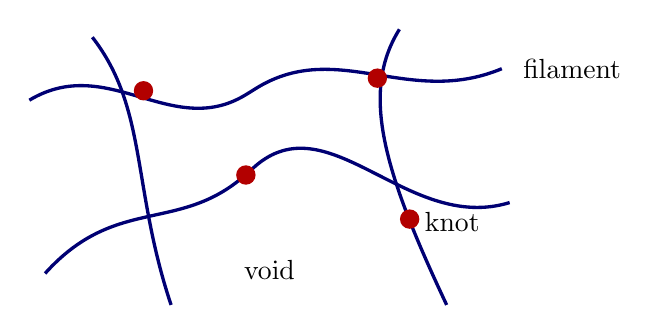
\begin{tikzpicture}[x=1cm,y=1cm]
  \draw[rounded corners=2pt,very thick,blue!45!black]
    (0.2,2.7) .. controls (1.2,3.3) and (2.0,2.2) .. (3.0,2.8)
    .. controls (4.1,3.5) and (5.0,2.6) .. (6.2,3.1);
  \draw[rounded corners=2pt,very thick,blue!45!black]
    (0.4,0.5) .. controls (1.3,1.5) and (2.1,1.0) .. (3.0,1.8)
    .. controls (4.0,2.7) and (5.0,1.0) .. (6.3,1.4);
  \draw[rounded corners=2pt,very thick,blue!45!black]
    (1.0,3.5) .. controls (1.7,2.6) and (1.5,1.6) .. (2.0,0.1);
  \draw[rounded corners=2pt,very thick,blue!45!black]
    (4.9,3.6) .. controls (4.4,2.8) and (4.7,1.8) .. (5.5,0.1);
  \fill[red!70!black] (1.65,2.82) circle (3.5pt);
  \fill[red!70!black] (4.62,2.98) circle (3.5pt);
  \fill[red!70!black] (2.95,1.75) circle (3.5pt);
  \fill[red!70!black] (5.03,1.19) circle (3.5pt);
  \node[align=center] at (3.25,0.55) {void};
  \node[right] at (6.35,3.1) {filament};
  \node[right] at (5.1,1.15) {knot};
\end{tikzpicture}
\caption{コースティック網の明快な二次元の類似。線状の集中がボイドを囲み、より明るい結び目で出会う。三次元では主な折り目はシートであり、その交差がフィラメントとノードを形成する。}
\label{fig:c09-caustic-network}
\end{figure}

無力の構成は宇宙論的摂動論の代替ではない。重力は密度コントラストの成長、ハロー形成、銀河、非線形構造にとって決定的である。この玩具模型は一つの頑健な幾何学的事実を分離する。すなわち、わずかに変化する初期の流れは自然に折り重なり集中する。小さな初期密度変動もまた、中心的なヤコビアンの議論を変えることなく含めることができる。

したがって、われわれは謎を解消したのではなく、移し替えたのである。インフレーションは、ある領域を極めて平坦で一様になるまで引き伸ばすために導入された。コースティックの計算は、微小な速度変動をもつ初期場を仮定している。その不均質な種はどこから来たのか。次の講義では、インフレーション中の場の量子揺らぎに目を向け、それらがどのようにして後の宇宙網の初期条件になるのかを問う。

\section{この議論が確立したこと}

一様なスカラー場は、ポテンシャル\(V(\phi)\)の中を運動する座標のように振る舞う。固定された箱の中では、それは\(\ddot\phi=-V'(\phi)\)に従う。膨張する共動的な箱の中では、物理的体積\(a^3\)が作用に現れ、
\[
\ddot\phi+3H\dot\phi=-V'(\phi).
\]
を生じる。ハッブル摩擦は、高く浅いポテンシャル上で場を遅い終端運動に保つことができる。そのときその運動エネルギーは無視できるようになり、そのポテンシャルエネルギーは\(H\)をほぼ一定に保ち、\(a(t)\)は近似的に指数関数的に成長する。

膨張は、望ましくないモノポールを希釈し、幾何を滑らかにし、曲率をゼロへと駆り立てる。それでもインフレーションは終わらなければならない。場はプラトーを離れ、振動し、そのエネルギーを再加熱の高温粒子へと移す。いくつかの問いは未解決のままである。ポテンシャルの形、インフラトンの正体と初期状態、その再加熱結合、そして今日観測される微小な真空エネルギーである。

インフレーションの成功は最後の問いを生む。完全に滑らかにされた宇宙には銀河が存在しないであろう。コースティック写像
\[
y=x+v(x)t,
\qquad
\frac{dn}{dy}=\frac{1}{1+v'(x)t}
\]
は、初期の流れにおける微小な変動が、どのようにして鋭いシート、フィラメント、結び目を生成しうるかを示す。それはそれらの変動の起源を説明しない。それらの量子的起源こそ、この議論が今から向かう主題である。
